\documentclass[tikz,border=10pt]{standalone}
\usepackage{tikz}
\usepackage{fontawesome5}
\usepackage{amsmath,amssymb}
\usetikzlibrary{arrows.meta,positioning,fit,backgrounds,calc,shadows,shapes.geometric}

\definecolor{civNavy}{RGB}{15, 34, 64}
\definecolor{civBlue}{RGB}{28, 80, 160}
\definecolor{civTeal}{RGB}{14, 130, 120}
\definecolor{civLightBlue}{RGB}{238, 245, 255}
\definecolor{civGold}{RGB}{217, 119, 6}
\definecolor{civGreen}{RGB}{22, 130, 80}
\definecolor{cInput}{RGB}{240, 246, 255}
\definecolor{cStem}{RGB}{224, 242, 254}
\definecolor{cStage1}{RGB}{209, 250, 229}
\definecolor{cStage2}{RGB}{254, 243, 199}
\definecolor{cStage3}{RGB}{254, 226, 226}
\definecolor{cStage4}{RGB}{236, 254, 255}

\begin{document}
% AI Vision Triage & Geospatial Routing Pipeline for CiviQ
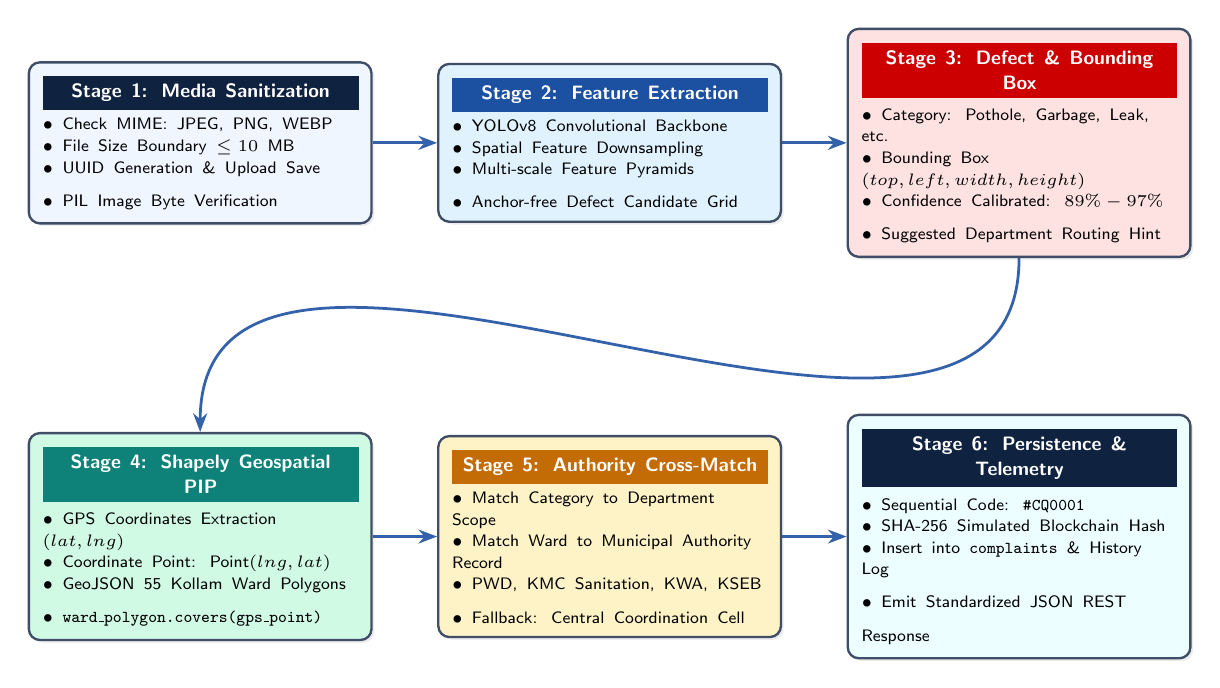
\begin{tikzpicture}[
    x=1cm, y=1cm,
    font=\sffamily,
    stagebox/.style={
        rectangle, draw=civNavy!80, line width=0.85pt, fill=white,
        rounded corners=4pt, inner sep=5pt, align=left,
        text width=4.0cm,
        drop shadow={shadow xshift=1pt, shadow yshift=-1pt, opacity=0.15}
    },
    flowarr/.style={
        -{Stealth[scale=0.9]}, line width=1.0pt, draw=civBlue!90
    }
]

    % STAGE 1
    \node [stagebox, fill=cInput] (s1) at (0, 7.5) {
        \colorbox{civNavy}{\parbox{3.8cm}{\centering\color{white}\bfseries\fontsize{7.5}{9.0}\selectfont Stage 1: Media Sanitization}}\\[3pt]
        \fontsize{6.5}{7.8}\selectfont
        $\bullet$ Check MIME: JPEG, PNG, WEBP\\
        $\bullet$ File Size Boundary $\le 10$ MB\\
        $\bullet$ UUID Generation \& Upload Save\\
        $\bullet$ PIL Image Byte Verification
    };

    % STAGE 2
    \node [stagebox, fill=cStem] (s2) at (5.2, 7.5) {
        \colorbox{civBlue}{\parbox{3.8cm}{\centering\color{white}\bfseries\fontsize{7.5}{9.0}\selectfont Stage 2: Feature Extraction}}\\[3pt]
        \fontsize{6.5}{7.8}\selectfont
        $\bullet$ YOLOv8 Convolutional Backbone\\
        $\bullet$ Spatial Feature Downsampling\\
        $\bullet$ Multi-scale Feature Pyramids\\
        $\bullet$ Anchor-free Defect Candidate Grid
    };

    % STAGE 3
    \node [stagebox, fill=cStage3] (s3) at (10.4, 7.5) {
        \colorbox{red!80!black}{\parbox{3.8cm}{\centering\color{white}\bfseries\fontsize{7.5}{9.0}\selectfont Stage 3: Defect \& Bounding Box}}\\[3pt]
        \fontsize{6.5}{7.8}\selectfont
        $\bullet$ Category: Pothole, Garbage, Leak, etc.\\
        $\bullet$ Bounding Box $(top, left, width, height)$\\
        $\bullet$ Confidence Calibrated: $89\% - 97\%$\\
        $\bullet$ Suggested Department Routing Hint
    };

    % STAGE 4
    \node [stagebox, fill=cStage1] (s4) at (0, 2.5) {
        \colorbox{civTeal}{\parbox{3.8cm}{\centering\color{white}\bfseries\fontsize{7.5}{9.0}\selectfont Stage 4: Shapely Geospatial PIP}}\\[3pt]
        \fontsize{6.5}{7.8}\selectfont
        $\bullet$ GPS Coordinates Extraction $(lat, lng)$\\
        $\bullet$ Coordinate Point: $\text{Point}(lng, lat)$\\
        $\bullet$ GeoJSON 55 Kollam Ward Polygons\\
        $\bullet$ \texttt{ward\_polygon.covers(gps\_point)}
    };

    % STAGE 5
    \node [stagebox, fill=cStage2] (s5) at (5.2, 2.5) {
        \colorbox{civGold!90!black}{\parbox{3.8cm}{\centering\color{white}\bfseries\fontsize{7.5}{9.0}\selectfont Stage 5: Authority Cross-Match}}\\[3pt]
        \fontsize{6.5}{7.8}\selectfont
        $\bullet$ Match Category to Department Scope\\
        $\bullet$ Match Ward to Municipal Authority Record\\
        $\bullet$ PWD, KMC Sanitation, KWA, KSEB\\
        $\bullet$ Fallback: Central Coordination Cell
    };

    % STAGE 6
    \node [stagebox, fill=cStage4] (s6) at (10.4, 2.5) {
        \colorbox{civNavy}{\parbox{3.8cm}{\centering\color{white}\bfseries\fontsize{7.5}{9.0}\selectfont Stage 6: Persistence \& Telemetry}}\\[3pt]
        \fontsize{6.5}{7.8}\selectfont
        $\bullet$ Sequential Code: \texttt{\#CQ0001}\\
        $\bullet$ SHA-256 Simulated Blockchain Hash\\
        $\bullet$ Insert into \texttt{complaints} \& History Log\\
        $\bullet$ Emit Standardized JSON REST Response
    };

    % Connecting Arrows
    \draw [flowarr] (s1) -- (s2);
    \draw [flowarr] (s2) -- (s3);
    \draw [flowarr] (s3.south) to[out=-90, in=90] (s4.north);
    \draw [flowarr] (s4) -- (s5);
    \draw [flowarr] (s5) -- (s6);

\end{tikzpicture}
\end{document}
